\documentclass[12pt, a4paper]{article}
\usepackage{../../../myconfig} % Gọi file cấu hình từ ngoài gốc vào

% ==========================================
% BẮT ĐẦU NỘI DUNG TÀI LIỆU
% ==========================================
\begin{document}

% Truyền 3 tham số: {Nhãn cam} {Chữ to chính giữa} {Chữ ở góc phải Header}
\titlebox{Chủ đề: Hàm số}{Đề kiểm tra định kì}{Hàm số: định kì}

\textit{\textbf{Phần I:} Thí sinh trả lời từ câu 1 đến câu 12, mỗi câu thí sinh chỉ chọn một phương án}

\vspace{0.5cm}

\questionLinesManual{0}{1}{Cho hàm số \( f(x) \) có bảng biến thiên như sau:
\begin{center}

\begin{tikzpicture}
\tkzTabInit[color, lgt=1.5, espcl=3.5]
{$x$ / 1, $f'(x)$ / 1, $f(x)$ / 2.5}
{$-\infty$, $-2$, $0$, $2$, $+\infty$}
\tkzTabLine{ , +, 0, -, 0, +, 0, - }
\tkzTabVar{-/$-\infty$, +/$3$, -/$2$, +/$3$, -/$-\infty$}
\end{tikzpicture}
\end{center}
Hàm số đã cho đồng biến trên khoảng nào dưới đây?}{%
\begin{tasks}(4)
\task \(( -\infty;3)\)
\task \((0; 2)\)
\task \((-2; 0)\)
\task \(( -\infty;-2)\cup(0;2)\)
\end{tasks}
}

\questionLinesManual{0}{2}{Cho hàm số \( f(x) \) liên tục trên \( \mathbb{R} \setminus \{1\} \) có bảng xét dấu như sau:
\begin{center}

\begin{tikzpicture}[>=stealth]
    \tkzTabInit[nocadre=false,lgt=1.2,espcl=2.5]
    {$x$ / 1, $f'(x)$ / 1}
    {$-\infty$, $1$, $3$, $+\infty$}
    \tkzTabLine{ , +, d, -, d, + }
\end{tikzpicture}
\end{center}
Hàm số có bao nhiêu điểm cực trị:}{%
\begin{tasks}(4)
\task 0
\task 1
\task 2
\task 3
\end{tasks}
}

\questionLinesManual{0}{3}{ Giá trị lớn nhất của hàm số \( f(x) = x^3 + 3x - 6 \) trên đoạn \([1; 3]\) là}{
    \begin{tasks}(4)
        \task $30$
        \task $39$
        \task $36$
        \task $10$
    \end{tasks}
}

\questionLinesManual{0}{4}{Đường cong bên là đồ thị hàm số nào sau đây?

\begin{center}
\begin{tikzpicture}[>=latex, scale=0.8]
    % 2. Vẽ hệ trục tọa độ
    \draw[->] (-3.5,0) -- (3.5,0) node[below] {\small $x$};
    \draw[->] (0,-3) -- (0,3.5) node[right] {\small $y$};
    \node[below left] at (0,0) {\small $O$};
    
    % 3. Vẽ đồ thị hàm số y = x^3 - 3x
    \draw[thick, samples=100, domain=-2.1:2.1] 
        plot (\x, {\x*\x*\x - 3*\x});
\end{tikzpicture}
\end{center}

}{
    \begin{tasks}(4)
        \task \( y = x^3 - 3x + 1 \)
        \task \( y = x^3 - 3x \)
        \task \( y = x^3 - 3x - 1 \)
        \task \( y = x^3 + 3x \)
    \end{tasks}
}

\questionLinesManual{0}{5}{Cho hàm số \( y = f(x) \) xác định trên \( \mathbb{R} \setminus \{1\} \), liên tục trên mỗi khoảng xác định và có bảng biến thiên hình vẽ sau

\begin{center}

\begin{tikzpicture}
    \tkzTabInit[lgt=1.5, espcl=3.5]
    {$x$ /1, $y'$ /1, $y$ /2.5}
    {$-\infty$, $1$, $+\infty$}
    \tkzTabLine{, -, d, -, }
    \tkzTabVar{+/ $1$ / , -D+/ $-\infty$ / $+\infty$ , -/ $1$ /}
\end{tikzpicture}
\end{center}

Bảng biến thiên trên là của hàm số nào trong các hàm số sau?}{
    \begin{tasks}(4)
        \task \( y = \dfrac{-x+2}{x-1} \)
        \task \( y = \dfrac{x+2}{x-1} \)
        \task \( y = \dfrac{x-3}{x-1} \)
        \task \( y = \dfrac{x+2}{x+1} \)
    \end{tasks}
}

\questionLinesManual{0}{6}{Cho hàm số \( y = f(x) \) có bảng biến thiên như sau

\begin{center}

\begin{tikzpicture}
    \tkzTabInit[lgt=1.5, espcl=2.5]
    {$x$ /1, $y'$ /1, $y$ /2.5}
    {$-\infty$, $-2$, $0$, $+\infty$}
    \tkzTabLine{, -, d, +, d, -, }
    \tkzTabVar{+/ $+\infty$ / , -D-/ $1$ / $-\infty$/ ,+D+/ $+\infty$ / $1$ , -/ $0$ /}
\end{tikzpicture}
\end{center}

Tổng số đường tiệm cận đứng và tiệm cận ngang của đồ thị hàm số đã cho bằng}{
    \begin{tasks}(4)
        \task $3$
        \task $2$
        \task $1$
        \task $4$
    \end{tasks}
}




\questionLinesManual{0}{7}{Cho hàm số \( y = ax^3 + 3x + d \) (\( a, d \in \mathbb{R} \)) có đồ thị như hình bên. Mệnh đề nào dưới đây đúng?

\begin{center}
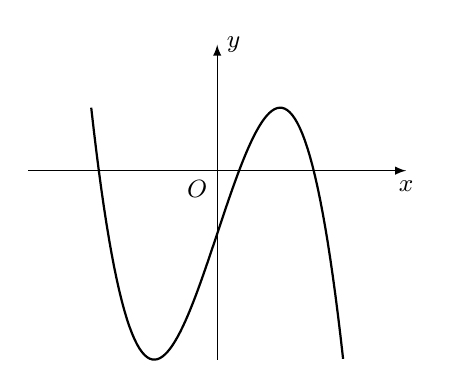
\begin{tikzpicture}[>=latex, scale=0.8]
    % Hệ trục tọa độ
    \draw[->] (-3,0) -- (3,0) node[below] {\small $x$};
    \draw[->] (0,-3) -- (0,2) node[right] {\small $y$};
    \node[below left] at (0,0) {\small $O$};   
    % Đồ thị hàm bậc 3: y = x^3 - 3x
    \draw[thick, samples=100, domain=-2:2] 
        plot (\x, {-\x*\x*\x + 3*\x-1});
   
\end{tikzpicture}
\end{center}

}{
    \begin{tasks}(4)
        \task \( a > 0, d > 0 \)
        \task \( a < 0, d > 0 \)
        \task \( a > 0, d < 0 \)
        \task \( a < 0, d < 0 \)
    \end{tasks}
}

\questionLinesManual{0}{8}{ Cho hàm số \( y = f(x) \) liên tục trên đoạn \([-1; 3]\) và có đồ thị như hình vẽ bên. Gọi \( M, m \) lần lượt là giá trị lớn nhất và giá trị nhỏ nhất của hàm số đã cho trên đoạn \([0; 3]\). Giá trị của \( M + m \) là

\begin{center}
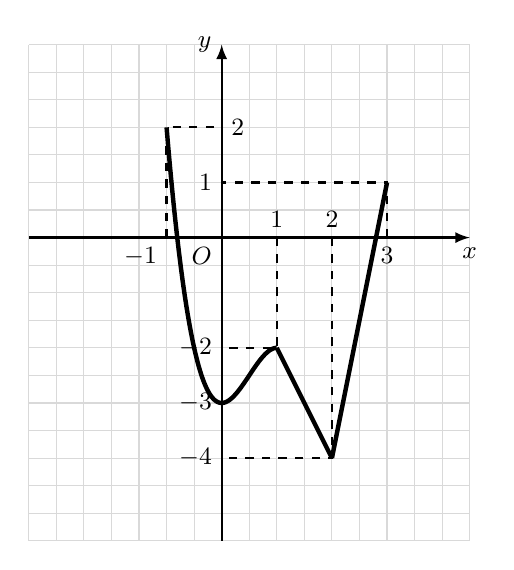
\begin{tikzpicture}[>=latex, scale=0.7]
    % 1. Vẽ lưới ô vuông (grid) màu xám nhạt phía sau đồ thị
    \draw[color=gray!30, thin, step=0.5] (-3.5,-5.5) grid (4.5,3.5);

    % 2. Hệ trục tọa độ Ox, Oy màu đen
    \draw[->, black, thick] (-3.5, 0) -- (4.5, 0) node[below] {\small $x$};
    \draw[->, black, thick] (0, -5.5) -- (0, 3.5) node[left] {\small $y$};
    \node[below left] at (0,0) {\small $O$};

    % 3. Đồ thị hàm số màu đen (black, ultra thick) từng nhánh
    % Nhánh 1: Đường cong mượt từ x = -1 (y = 2) qua (0, -3) đến cực đại (1, -2)
    \draw[black, ultra thick, samples=100, domain=-1:1] plot (\x, {-2*\x*\x*\x + 3*\x*\x - 3});
    
    % Nhánh 2: Đoạn thẳng từ (1, -2) xuống (2, -4)
    \draw[black, ultra thick] (1,-2) -- (2,-4);
    
    % Nhánh 3: Đoạn thẳng từ (2, -4) lên điểm mút (3, 1)
    \draw[black, ultra thick] (2,-4) -- (3,1);

    % 4. Các đường nét đứt và nhãn tọa độ màu đen
    % Tại x = -1, y = 2
    \draw[dashed, black, thick] (-1,0) -- (-1,2) -- (0,2);
    \node[below left] at (-1,0) {\small $-1$};
    \node[right] at (0,2) {\small $2$};
    
    % Mốc y = -3 và y = 1 trên Oy
    \node[left] at (0,-3) {\small $-3$};
    \node[left] at (0,1) {\small $1$};
    
    % Tại x = 1, y = -2
    \draw[dashed, black, thick] (1,0) -- (1,-2) -- (0,-2);
    \node[above] at (1,0) {\small $1$};
    \node[left] at (0,-2) {\small $-2$};
    
    % Tại x = 2, y = -4
    \draw[dashed, black, thick] (2,0) -- (2,-4) -- (0,-4);
    \node[above] at (2,0) {\small $2$};
    \node[left] at (0,-4) {\small $-4$};
    
    % Tại x = 3, y = 1
    \draw[dashed, black, thick] (3,0) -- (3,1) -- (0,1);
    \node[below] at (3,0) {\small $3$};

\end{tikzpicture}
\end{center}

}{
    \begin{tasks}(4)
        \task $2$
        \task $-3$
        \task $-5$
        \task $-2$
    \end{tasks}
}

\questionLinesManual{0}{9}{Tập nghiệm của bất phương trình \( \log_7(x-3) \leq 1 \) là:}{
    \begin{tasks}(4)
        \task $[3; 10]$
        \task $(3; 10]$
        \task $(3; 10)$
        \task $[3; 10)$
    \end{tasks}
}

\questionLinesManual{0}{10}{Đường cong như hình vẽ dưới đây là đồ thị của hàm số nào?

\begin{center}
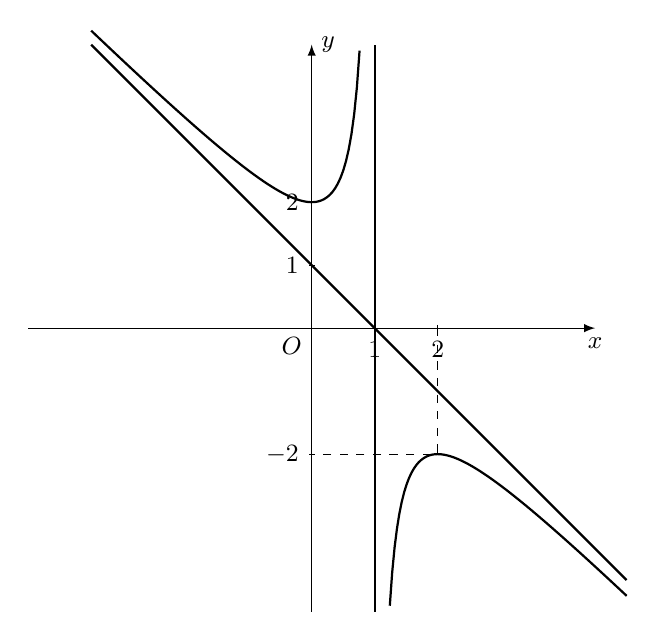
\begin{tikzpicture}[>=latex, scale=0.8]
    % 1. Hệ trục tọa độ
    \draw[->] (-4.5,0) -- (4.5,0) node[below] {\small $x$};
    \draw[->] (0,-4.5) -- (0,4.5) node[right] {\small $y$};
    \node[below left] at (0,0) {\small $O$};
    
    % 2. Đánh dấu các mốc
    \foreach \x in {1,2} {
        \draw (\x,0.05) -- (\x,-0.05) node[below] {\small $\x$};
    }
    \foreach \val in {-2,1,2} {
        \draw (0.05,\val) -- (-0.05,\val) node[left] {\small $\val$};
    }
    
    % 3. Vẽ đồ thị hàm số y = (-x^2 + 2x - 2)/(x-1)
    \draw[thick, samples=100, domain=-3.5:0.76] 
        plot (\x, {(-\x*\x + 2*\x - 2)/(\x - 1)});
    \draw[thick, samples=100, domain=1.24:5] 
        plot (\x, {(-\x*\x + 2*\x - 2)/(\x - 1)});
     \draw[thick, samples=100, domain=-3.5:5] 
        plot (\x, {(-\x+1});
    % 4. Đường tiệm cận
    \draw[thick] (1,-4.5) -- (1,4.5);
    \draw [dashed] (2,0) -- ( 2,-2) -- ( 0,-2);
\end{tikzpicture}
\end{center}

}{
    \begin{tasks}(4)
        \task \( y = \dfrac{x-2}{x-1} \)
        \task \( y = \dfrac{x^2 + 2x - 2}{x-1} \)
        \task \( y = \dfrac{-x^2 + 2x - 2}{x-1} \)
        \task \( y = \dfrac{-x^2 + x - 2}{x-1} \)
    \end{tasks}
}
\questionLinesManual{0}{11}{Cho cấp số nhân \( (u_n) \) có số hạng đầu \( u_1 = 5 \) và công bội \( q = -2 \). Số hạng thứ sáu của \( (u_n) \) là:}{
    \begin{tasks}(4)
        \task \( u_6 = -320 \)
        \task \( u_6 = 320 \)
        \task \( u_6 = 160 \)
        \task \( u_6 = -160 \)
    \end{tasks}
}

\questionLinesManual{0}{12}{Cho hàm số \( y = f(x) \) liên tục trên \( \mathbb{R} \) và có đạo hàm  
\( f'(x) = (x+1)^3(x^2-1)(x-2)^2. \) 
Số điểm cực trị của hàm số đã cho là}{%
\begin{tasks}(4)
\task 1
\task 3
\task 2
\task 0
\end{tasks}
}

\textit{\textbf{Phần II:} Thí sinh trả lời từ câu 13 đến câu 16; trong mỗi ý a), b), c), d) ở mỗi câu, thí sinh chọn đúng hoặc sai.}

\vspace{0.3cm}
%Câu 75
\questionTrueFalse{0}{13}{Cho hàm số \( y = f(x) = x^3 - 3x + 2 \) có đồ thị \( (C) \) và đường thẳng \( (d) \): \( y = 9x + 18 \). Biết đường thẳng \( (d) \) là tiếp tuyến của đồ thị \( (C) \) tại điểm \( M(x_0; y_0) \).}{
    \textbf{a)} & Đạo hàm của hàm số là \( f'(x) = x^2 - 3 \).
    & \textcolor{amberorange}{$\bigcirc$} & \textcolor{amberorange}{$\bigcirc$} \\ \hline
    
    \textbf{b)} & Hệ số góc của tiếp tuyến tại điểm \( M \) là \( f'(x_0) = 9 \).
    & \textcolor{amberorange}{$\bigcirc$} & \textcolor{amberorange}{$\bigcirc$} \\ \hline
    
    \textbf{c)} & Giá trị \( y_0 - x_0 = -2 \).
    & \textcolor{amberorange}{$\bigcirc$} & \textcolor{amberorange}{$\bigcirc$} \\ \hline
    
    \textbf{d)} & Số điểm chung của đồ thị \( (C) \) và đường thẳng \( (d) \) là hai.
    & \textcolor{amberorange}{$\bigcirc$} & \textcolor{amberorange}{$\bigcirc$} \\
}

% --- CÂU 79: ĐỒ THỊ f'(x) ---
\questionTrueFalse{0}{14}{ Cho hàm số \( y = f(x) \) có đạo hàm liên tục trên \( \mathbb{R} \). Hàm số \( y = f'(x) \) có đồ thị như hình dưới đây.

\begin{center}
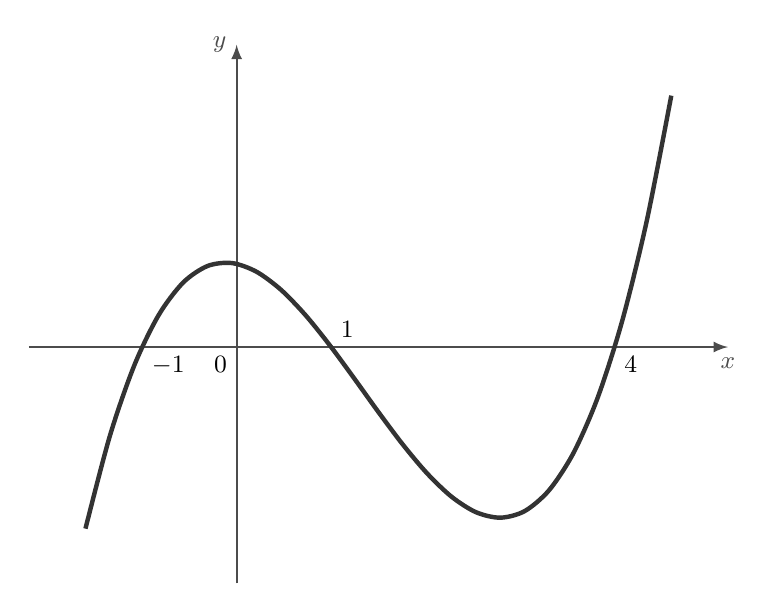
\begin{tikzpicture}[>=latex, scale=1.2]
    % 1. Hệ trục tọa độ Ox, Oy màu xám đậm
    \draw[->, black!70, thick] (-2.2, 0) -- (5.2, 0) node[below] {\small $x$};
    \draw[->, black!70, thick] (0, -2.5) -- (0, 3.2) node[left] {\small $y$};
    \node[below left] at (0,0) {\small $0$};
    
    % 2. Các nhãn tọa độ trên trục hoành Ox
    \node[below right] at (-1, 0) {\small $-1$};
    \node[above right] at (1, 0) {\small $1$};
    \node[below right] at (4, 0) {\small $4$};
    
    % 3. Đồ thị hàm số bậc ba (màu xám đen, nét dày)
    % Công thức mô phỏng chính xác tỉ lệ: y = 0.22 * (x + 1) * (x - 1) * (x - 4)
    \draw[black!80, ultra thick, smooth, domain=-1.6:4.6] 
        plot (\x, {0.22*(\x+1)*(\x-1)*(\x-4)});

\end{tikzpicture}
\end{center}

}{
    \textbf{a)} & Hàm số \( y = f(x) \) đồng biến trên khoảng \( (1; +\infty) \).
    & \textcolor{amberorange}{$\bigcirc$} & \textcolor{amberorange}{$\bigcirc$} \\ \hline
    
    \textbf{b)} & Trên đoạn \([-1; 4]\) thì giá trị lớn nhất của hàm số \( y = f(x) \) là \( f(1) \).
    & \textcolor{amberorange}{$\bigcirc$} & \textcolor{amberorange}{$\bigcirc$} \\ \hline
    
    \textbf{c)} & \( f(1) > f(2) > f(4) \).
    & \textcolor{amberorange}{$\bigcirc$} & \textcolor{amberorange}{$\bigcirc$} \\ \hline
    
    \textbf{d)} & Hàm số \( y = f(x) \) có hai cực trị.
    & \textcolor{amberorange}{$\bigcirc$} & \textcolor{amberorange}{$\bigcirc$} \\
}

% --- CÂU 1 BTVN ---
\questionTrueFalse{0}{15}{Tiệm vải bà Trâu đang tính toán các chi phí để vận hành xưởng và sản xuất \( x \) mét vải trong một tháng. Bà Trâu chia chi phí thành 3 hạng mục chính: chi phí thuê xưởng là 8 triệu đồng, chi phí nguyên liệu để sản xuất một mét vải là 25 nghìn đồng, và chi phí bảo trì máy móc là \( 0,00001x^2 \) triệu đồng. Biết rằng giá vải tiệm yết của tiệm vải bà Trâu là 100 nghìn đồng/mét vải và giả sử toàn bộ số vải sản xuất được thì đều được bán hết.}{
    \textbf{a)} & Tổng chi phí vận hành và sản xuất vải của tiệm vải bà Trâu trong một tháng được tính bằng công thức  
    \( C(x) = 0,00001x^2 + 0,025x + 8 \) (đơn vị: triệu đồng).
    & \textcolor{amberorange}{$\bigcirc$} & \textcolor{amberorange}{$\bigcirc$} \\ \hline
    
    \textbf{b)} & Nếu mỗi tháng tiệm vải bà Trâu sản xuất được 109m vải, khi đó tiệm sẽ bị lỗ.
    & \textcolor{amberorange}{$\bigcirc$} & \textcolor{amberorange}{$\bigcirc$} \\ \hline
    
    \textbf{c)} & Lợi nhuận lớn nhất mà tiệm vải bà Trâu có thể đạt được trong một tháng lớn hơn 132 triệu đồng.
    & \textcolor{amberorange}{$\bigcirc$} & \textcolor{amberorange}{$\bigcirc$} \\ \hline
    
    \textbf{d)} & Giả sử tiệm vải bà Trâu sản xuất số mét vải tiến đến vô cùng, khi đó chi phí trung bình để sản xuất mỗi mét vải sẽ tiến đến 0.
    & \textcolor{amberorange}{$\bigcirc$} & \textcolor{amberorange}{$\bigcirc$} \\
}

% --- CÂU 2 Bài Giảng ---
\questionTrueFalse{0}{16}{Để khắc phục tình trạng thất nghiệp tại quốc gia X, chính phủ của quốc gia này quyết định sẽ đưa ra các gói trợ cấp để tuyển dụng những người đang thất nghiệp vào làm việc cho các dự án của chính phủ.  
Giả sử rằng sau \( t \) tháng kể từ khi triển khai việc cung cấp các gói trợ cấp, khi đó quốc gia X có  
\(N(t) = -t^3 + 45t^2 + 408t + 3078\) 
người thất nghiệp. Cho biết rằng việc cung cấp các gói trợ cấp này được triển khai trong 4 năm.}{
    \textbf{a)} & Sau 3 năm kể từ khi triển khai việc cung cấp các gói trợ cấp, quốc gia X có 4680 người thất nghiệp.
    & \textcolor{amberorange}{$\bigcirc$} & \textcolor{amberorange}{$\bigcirc$} \\ \hline
    
    \textbf{b)} & Trong thời gian triển khai việc cung cấp các gói trợ cấp, số người thất nghiệp nhiều nhất tại cùng một thời điểm là 29699 người.
    & \textcolor{amberorange}{$\bigcirc$} & \textcolor{amberorange}{$\bigcirc$} \\ \hline
    
    \textbf{c)} & Sau 1 năm kể từ khi triển khai việc cung cấp các gói trợ cấp, tốc độ tăng số người thất nghiệp tại thời điểm đó là 1056 người/tháng.
    & \textcolor{amberorange}{$\bigcirc$} & \textcolor{amberorange}{$\bigcirc$} \\ \hline
    
    \textbf{d)} & Số người thất nghiệp tại quốc gia X tăng nhanh nhất sau 1 năm 3 tháng kể từ khi triển khai việc cung cấp các gói trợ cấp.
    & \textcolor{amberorange}{$\bigcirc$} & \textcolor{amberorange}{$\bigcirc$} \\
}

\textit{\textbf{Phần III:} Thí sinh trả lời từ câu 17 đến câu 22.}

\vspace{0.3cm}

\questionShortAnswer{0}{17}{Trong 5 giây đầu tiên, một chất điểm chuyển động theo phương trình \( s(t) = t^3 - 3t^2 + 8t + 2 \). Trong đó, \( t \) tính bằng giây và \( s \) tính bằng mét. Chất điểm có vận tốc tức thời nhỏ nhất bằng bao nhiêu \( m/s \) trong 5 giây đầu tiên đó?}

\questionShortAnswer{0}{18}{Bạn Trân Đầu có một mảnh đất rộng và muốn dành ra một khu đất hình chữ nhật có diện tích 288 m² để trồng vài loại cây mới. Bạn dự kiến rào quanh ba cạnh của khu đất hình chữ nhật này bằng lưới thép, cạnh còn lại (chiều dài) sẽ tận dụng bức tường có sẵn (hình vẽ). Do điều kiện địa lí, chiều rộng khu đất không vượt quá 18 m, hỏi chiều dài của khu đất này bằng bao nhiêu mét để tổng chiều dài lưới thép cần dùng là ngắn nhất (nghĩa là chi phí rào lưới thép thấp nhất)?

\begin{center}
\begin{tikzpicture}[>=latex, scale=0.8]
   \begin{scope}[xshift=0cm, yshift=0cm]
        \node[anchor=south west, inner sep=0] at (0,0) {
            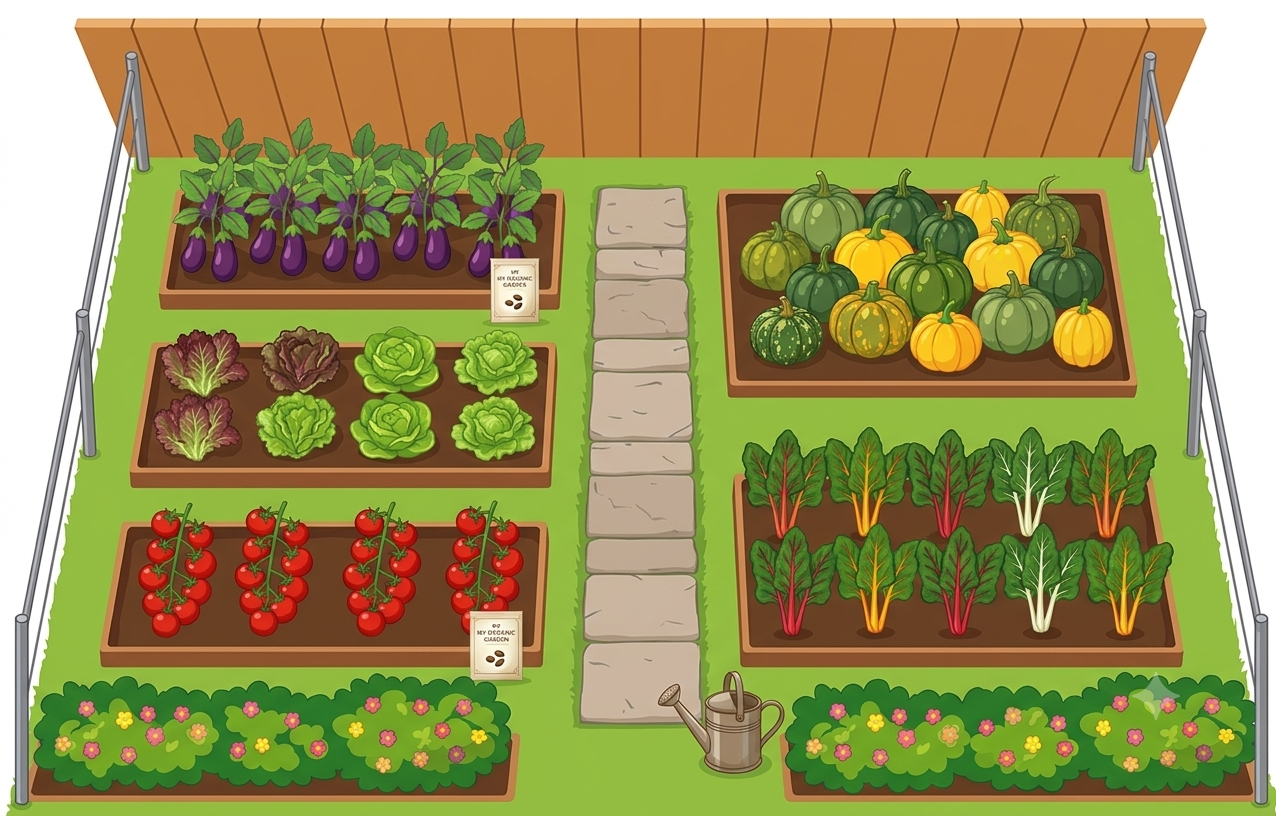
\includegraphics[width=5cm]{images/NongTrai.png}
        };
    \end{scope}
\end{tikzpicture}
\end{center}}

\questionShortAnswer{0}{19}{Bác Thúy có một bãi nuôi cá, mỗi ngày thu hoạch được 1 tấn cá. Nếu bác bán cho thương lái với giá 30 nghìn đồng/kg thì hết cá, nếu giá bán cứ tăng thêm 5 nghìn đồng/kg thì số cá thừa sẽ tăng thêm 20kg. Số cá thừa này được bán để làm thức ăn cho động vật với giá 10 nghìn đồng/kg. Hỏi doanh thu lớn nhất từ việc bán cá mỗi ngày của bác Thúy là bao nhiêu triệu đồng?}

% --- CÂU 8 BTVN ---
\questionShortAnswer{0}{20}{Một người chèo một chiếc thuyền xuất phát từ điểm \( A \) trên bờ một con sông thẳng rộng \( 3,5 \, \text{km} \), và muốn đến điểm \( B \) cách điểm \( C \) \( 7 \, \text{km} \). Người này có thể chèo thuyền qua sông đến điểm \( C \) rồi chạy bộ đến \( B \), hoặc anh ta có thể chèo thuyền thẳng đến \( B \). Hoặc anh ta có thể chèo thuyền qua sông đến điểm \( D \) nào đó giữa \( C \) và \( B \) rồi chạy đến điểm \( B \) (hình minh họa).

\begin{center}
\begin{tikzpicture}[>=stealth, scale=1.3]

    % =================================================================
    % 1. ĐỊNH NGHĨA TỌA ĐỘ CÁC ĐIỂM CHÍNH
    % =================================================================
    \coordinate (A) at (1.5, 0);
    \coordinate (C) at (1.5, 2.2);
    \coordinate (D) at (3.2, 2.2);
    \coordinate (B) at (8.5, 2.2);
    
    % Giới hạn hai bờ sông kéo dài sang hai bên
    \coordinate (TopLeft) at (0.2, 2.2);
    \coordinate (TopRight) at (8.8, 2.2);
    \coordinate (BottomLeft) at (0.2, 0);
    \coordinate (BottomRight) at (8.8, 0);

    % =================================================================
    % 2. VẼ NỀN DÒNG SÔNG (HỌA TIẾT SÓNG NƯỚC)
    % =================================================================
    \foreach \x in {0.3, 0.8, 1.3, 1.8, 2.3, 2.8, 3.3, 3.8, 4.3, 4.8, 5.3, 5.8, 6.3, 6.8, 7.3, 7.8, 8.3} {
        \foreach \y in {0.2, 0.5, 0.8, 1.1, 1.4, 1.7, 2.0} {
            \draw[shift={(\x,\y)}, xscale=0.5, yscale=0.3, thin, gray!60] 
                (0,0) sin (0.2,0.2) cos (0.4,0) sin (0.6,-0.2) cos (0.8,0);
        }
    }

    % Vẽ hai đường biên song song của bờ sông
    \draw[thick] (TopLeft) -- (TopRight);
    \draw[thick] (BottomLeft) -- (BottomRight);

    % =================================================================
    % 3. VẼ CÁC VECTOR DI CHUYỂN QUA SÔNG
    % =================================================================
    \draw[->, very thick] (A) -- (C);
    \draw[->, very thick] (A) -- (D);
    \draw[->, very thick] (A) -- (B);

    % =================================================================
    % 4. VẼ BIỂU TƯỢNG NGƯỜI CHÈO THUYỀN TẠI VỊ TRÍ A
    % =================================================================
    \begin{scope}[shift={(A)}, scale=0.45, xshift=-1.8cm, yshift=0.2cm]
        % Sóng nước nhỏ dưới thuyền
        \draw[thin] (-0.2,-0.2) sin (0.2,-0.3) cos (0.6,-0.2) sin (1.0,-0.3);
        % Thân thuyền
        \draw[thick, fill=white] (0,0.2) -- (2.0,0.2) -- (1.7,-0.2) -- (0.3,-0.2) -- cycle;
        \draw[thick] (0,0.2) -- (2.0,0.2);
        % Người chèo thuyền
         \draw[thick] (1,0.8) circle (5pt); % Đầu
        \draw[thick] (1.0,0.65) -- (1.0,0.2); % Thân
        \draw[thick] (1.0,0.5) -- (0.6,0.3) -- (0.8,0.0); % Tay giữ mái chèo
        \draw[thick] (1.0,0.5) -- (1.3,0.3); 
        % Mái chèo
        \draw[thick] (0.4,-0.1) -- (1.4,0.7);
    \end{scope}

    % =================================================================
    % 5. GÁN NHÃN CÁC ĐỈNH VÀ CHÚ THÍCH CHỮ
    % =================================================================
    \node[below=4pt] at (A) {$A$};
    \node[above=4pt] at (C) {$C$};
    \node[above=4pt] at (D) {$D$};
    \node[above=4pt] at (B) {$B$};

    % Độ dài khoảng cách chiều rộng sông
    \node[left=3pt] at (1.5, 1.4) {$3,5km$};

    % Chú thích địa hình "bờ sông" ở trên và dưới
    \node[above] at (5.0, 2.2) {bờ sông};
    \node[below] at (5.0, 0) {bờ sông};

\end{tikzpicture}
\end{center}

Biết rằng vận tốc chèo thuyền của anh ta là \( 5 \, \text{km/h} \) (đã tính vận tốc nước), vận tốc chạy bộ của anh ta là \( 9 \, \text{km/h} \). Trong tất cả các phương án đến \( B \) bằng cách chèo thuyền hoặc chèo thuyền rồi chạy bộ, phương án nhanh nhất có tổng thời gian là bao nhiêu giờ (kết quả làm tròn đến hàng phần trăm)?}
%Câu 3 bài giảng
\questionShortAnswer{0}{21}{Lát cắt ngang của một vùng đất được mô hình hóa là một phần hàm số bậc ba \( y = f(x) \) có đồ thị như hình vẽ (đơn vị độ dài trên các trục là kilômét). Biết khoảng cách hai bên chân đồi \( OM = 4 \, (km) \), độ rộng của hồ nước \( MN = 2 \, (km) \) và ngọn đồi cao \( 1056 \, (m) \). Độ sâu của hồ nước là bao nhiêu mét (làm tròn kết quả đến hàng đơn vị của mét)?

\begin{center}
\begin{tikzpicture}[>=stealth, scale=1.2]

    % Phần Đồi: Giới hạn bởi trục hoành và đường cong từ x=0 đến x=4 (Họa tiết ca-rô mắt cáo)
    \path[pattern=grid, pattern color=gray!80] (0,0) -- plot[domain=0:4, samples=100] (\x, {0.15*\x*(\x-4)*(\x-6)}) -- (4,0) -- cycle;

    % Phần Hồ Nước: Giới hạn bởi trục hoành và đường cong từ x=4 đến x=6 (Họa tiết sọc chéo)
    \path[pattern=north west lines, pattern color=gray!80] (4,0) -- plot[domain=4:6, samples=100] (\x, {0.15*\x*(\x-4)*(\x-6)}) -- (6,0) -- cycle;

    % Phần Núi: Giới hạn bởi trục hoành, đường cong từ x=6 đến x=7.1 và trục đứng bên phải x=7.1 (Họa tiết mắt cáo)
    \path[pattern=grid, pattern color=gray!80] (6,0) -- plot[domain=6:7.1, samples=100] (\x, {0.15*\x*(\x-4)*(\x-6)}) -- (7.1,0) -- cycle;

    % =================================================================
    % 2. VẼ ĐƯỜNG BIÊN ĐỒ THỊ VÀ HỆ TRỤC TỌA ĐỘ Oxy
    % =================================================================
    % Trục hoành Ox và Trục tung Oy
    \draw[->, thick] (-0.8, 0) -- (8.0, 0) node[below] {$x$};
    \draw[->, thick] (0, -1.0) -- (0, 3.2) node[left] {$y$};
    \node[below left] at (0,0) {$O$};

    % Đường biên giới hạn bên phải của núi
    \draw[thick] (7.1, 0) -- (7.1, {0.15*7.1*(7.1-4)*(7.1-6)});

    % Vẽ toàn bộ đường cong hàm số bậc ba liên tục
    \draw[ultra thick, samples=150, domain=0:7.1] plot (\x, {0.15*\x*(\x-4)*(\x-6)});

    % =================================================================
    % 3. CHÚ THÍCH CÁC ĐỊA DANH VÀ ĐIỂM SỐ
    % =================================================================
    \node[below=3pt] at (4, 0) {$M$};
    \node[below=3pt] at (6, 0) {$N$};

    % Tên địa danh tương ứng trên đồ thị
    \node[above, scale=0.85] at (1.6, 2.5) {Đồi};
    \node[above, scale=0.85] at (5.0, 0.05) {Mặt hồ};
    \node[left, scale=0.85] at (6.6, 1.8) {Núi};

\end{tikzpicture}
\end{center}}

% --- CÂU 1 ---
\questionShortAnswer{0}{22}{Một cái máng dạng hình lăng trụ, trong đó hai đầu của máng là tam giác cân, với đáy 3 m và chiều cao 4 m, và chiều dài của máng là 10 m. Nước đang được bơm vào máng với tốc độ \( 5 \, \text{m}^3 / \text{phút} \). Hỏi tốc độ thay đổi chiều cao của mực nước là bao nhiêu m/phút khi mực nước đang ở độ cao 1 m? (Kết quả làm tròn đến hàng phần trăm).
\begin{figure}[htbp]
    
    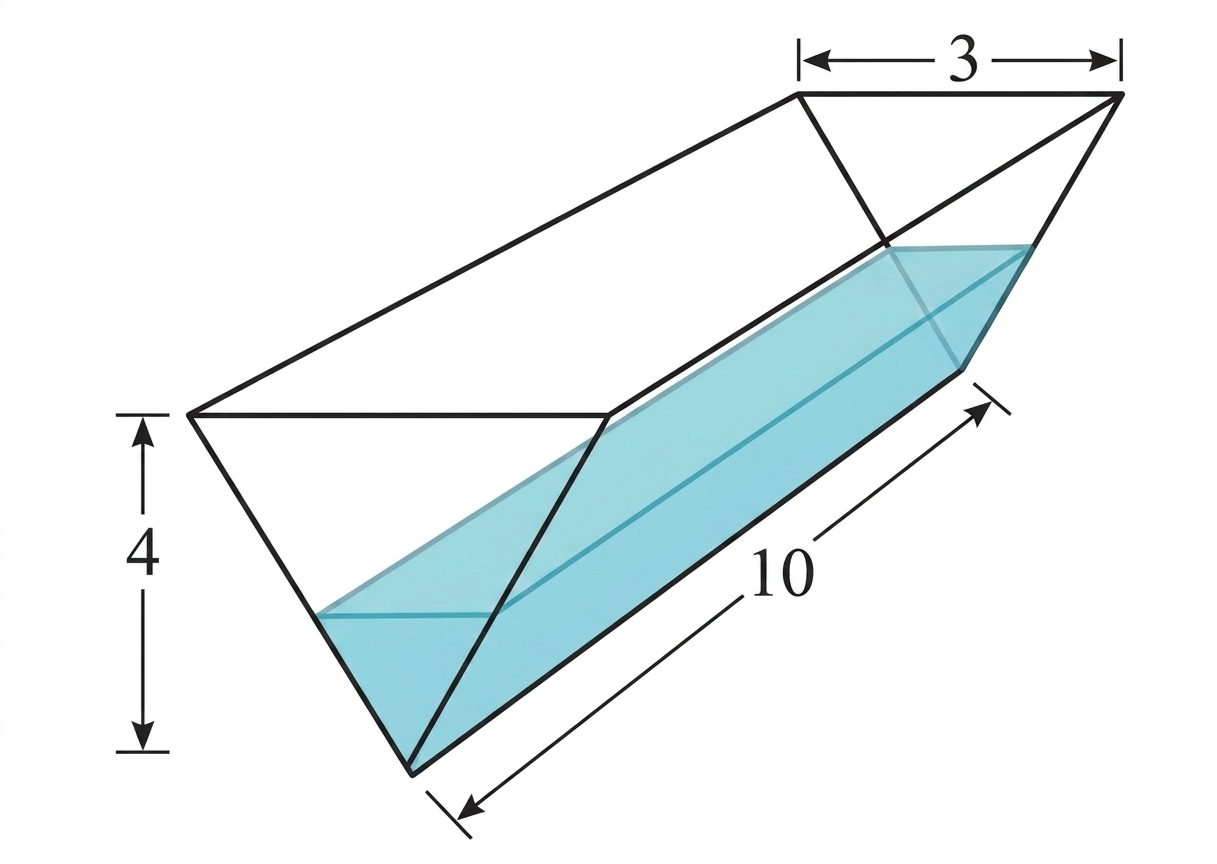
\includegraphics[width=0.4\textwidth]{images/Cau1nuocdang.png}
    
\end{figure}

}

\end{document}